\chapter{Asam, Basa, dan pH}\label{ch:g9:acids-bases-ph}

Di rak dapur berjajar sebutir jeruk lemon, sebotol cuka, sebatang sabun,
dan sekotak soda kue; di bawah bak cuci, sebotol pembersih saluran
dengan label peringatan hitam-merah. Sebagian terasa asam, sebagian
terasa licin, sebagian dapat melukai kulit. Satu skala saja, bernomor
dari 0 sampai 14, memilah semuanya --- dan skala yang sama dipakai untuk
kolam renang, tanah kebun, darah, dan samudra.

\begin{recall}
\omterm{def:g9:ions:ion}{Ion} adalah \omterm{def:g7:atoms-and-molecules:atom}{atom} atau sekelompok \omterm{def:g7:atoms-and-molecules:atom}{atom} yang bermuatan; \omterm{def:g9:ions:ion}{kation} seperti
\ce{Na+} bermuatan positif, \omterm{def:g9:ions:ion}{anion} seperti \ce{Cl-} atau \ce{OH-}
bermuatan negatif. Larutan \omterm{def:g9:ions:ion}{ion} mengandung \omterm{def:g9:ions:ion}{ion-ion} bertanda (aq), yang
bergerak bebas (\cref{ch:g9:ions}).
\end{recall}

\begin{omfigure}
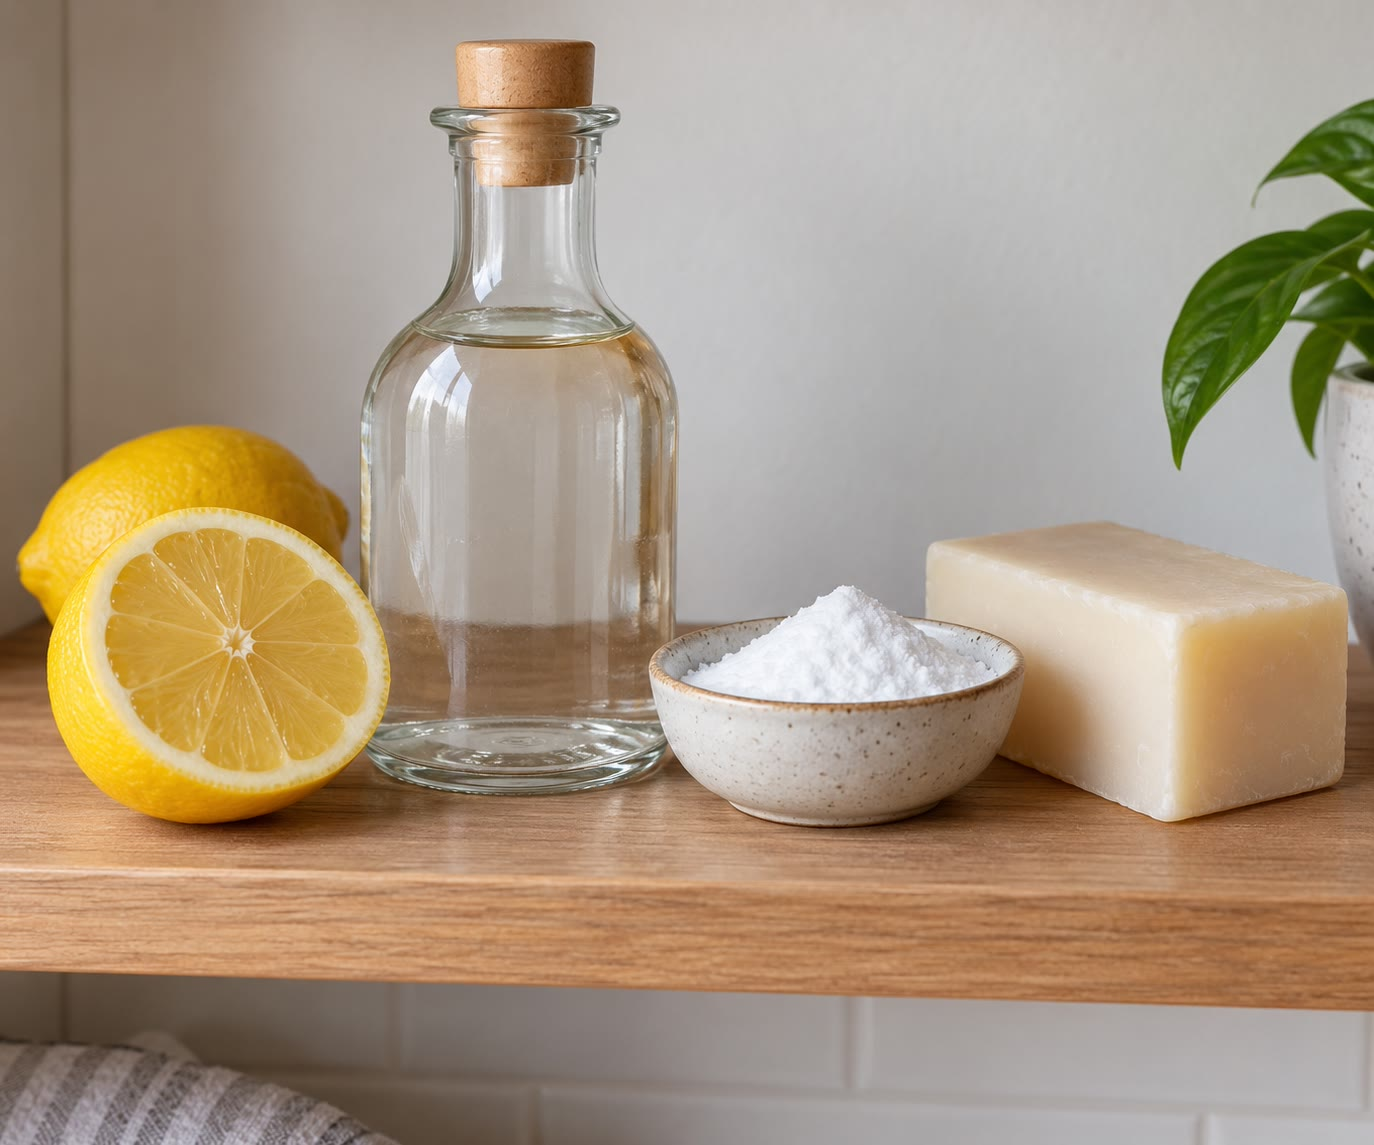
\includegraphics[width=0.55\linewidth]{images/book1/ai/g9-kitchen-shelf.jpg}

{\small Jeruk lemon, cuka, sabun, dan soda kue: asam dan basa di
dapur.}
\end{omfigure}

\section{Larutan asam, basa, dan netral}

\begin{definition}[Larutan asam, basa, dan netral]\label{def:g9:acids-bases-ph:acidic}
Setiap \omterm{def:g6:solutions-and-solubility:solute}{larutan berair} mengandung \omterm{def:g9:ions:ion}{ion} hidrogen \ce{H+(aq)} dan \omterm{def:g9:ions:ion}{ion}
hidroksida \ce{OH-(aq)}. Sebuah larutan disebut
\emph{larutan asam}\index{larutan asam} jika mengandung lebih banyak \omterm{def:g9:ions:ion}{ion}
\ce{H+} daripada \omterm{def:g9:ions:ion}{ion} \ce{OH-}, \emph{larutan basa}\index{larutan basa}
jika mengandung lebih banyak \omterm{def:g9:ions:ion}{ion} \ce{OH-} daripada \omterm{def:g9:ions:ion}{ion} \ce{H+}, dan
\emph{larutan netral}\index{larutan netral} jika jumlah keduanya sama.
\end{definition}

\begin{example}[Tiga larutan]\label{ex:g9:acids-bases-ph:three}
Asam klorida adalah \omterm{def:g9:acids-bases-ph:acidic}{larutan asam}: larutan itu mengandung \omterm{def:g9:ions:ion}{ion}
\ce{H+(aq)} dan \ce{Cl-(aq)}, dengan sangat sedikit \ce{OH-}. Larutan
natrium hidroksida bersifat basa: \ce{Na+(aq)} dan \ce{OH-(aq)}, dengan
sangat sedikit \ce{H+}. Air murni dan air garam netral.
\end{example}

\section{Skala pH}

\begin{definition}[pH]\label{def:g9:acids-bases-ph:ph}
Yang disebut \emph{pH}\index{pH} sebuah \omterm{def:g6:solutions-and-solubility:solute}{larutan berair} adalah sebuah
bilangan, biasanya antara 0 dan 14, yang menyatakan seberapa asam atau
basa larutan itu: pada \qty{25}{\celsius}, \omterm{def:g9:acids-bases-ph:acidic}{larutan netral} memiliki pH 7,
\omterm{def:g9:acids-bases-ph:acidic}{larutan asam} pH di bawah 7, \omterm{def:g9:acids-bases-ph:acidic}{larutan basa} pH di atas 7. Makin banyak \omterm{def:g9:ions:ion}{ion}
\ce{H+} yang dikandung sebuah larutan, makin rendah pH-nya.
\end{definition}

\begin{omfigure}
\begin{tikzpicture}[font=\small, x=0.95cm]
  \foreach \k in {0,...,13} {
    \pgfmathtruncatemacro\rr{2.2*max(0,100-14.3*\k)+30}
    \pgfmathtruncatemacro\gg{1.8*(\k<7 ? 30+10*\k : 100-8*(\k-7))+40}
    \pgfmathtruncatemacro\bb{2.2*max(0,14.3*(\k-6))+30}
    \definecolor{phc}{RGB}{\rr,\gg,\bb}
    \fill[phc] (\k,0) rectangle ++(1,0.6);
  }
  \foreach \k in {0,...,14} \node[anchor=north, font=\footnotesize] at (\k,-0.02) {\k};
  \draw[black!60] (0,0) rectangle (14,0.6);
  \node[anchor=south] at (3.5,0.65) {asam};
  \node[anchor=south] at (7,0.65) {netral};
  \node[anchor=south] at (10.5,0.65) {basa};
  % ledger: ph:HCl-1M, ph:gastric, ph:lime, ph:wine, ph:coffee, ph:pure-water, ph:seawater, ph:milk-magnesia, ph:ammonia, ph:NaOH-1M
  \foreach \x/\lab/\lev/\anc in {0/{asam klorida\\ (1 M)}/1/north, 1.5/{cairan\\ lambung}/3/north east,
      2/{air jeruk\\ nipis}/2/north west, 3.5/{anggur}/1/north, 5/{kopi}/2/north, 7/{air\\ murni}/3/north,
      8.1/{air\\ laut}/1/north, 10.5/{susu\\ magnesia}/3/north, 12/{amonia\\ rumah tangga}/1/north,
      14/{natrium hidroksida\\ (1 M)}/2/north east} {
    \draw[black!55] (\x,-0.45) -- (\x,-0.45-0.8*\lev);
    \node[anchor=\anc, font=\footnotesize, align=center, inner sep=2pt] at (\x,-0.45-0.8*\lev) {\lab};
  }
\end{tikzpicture}

{\small Skala \omterm{def:g9:acids-bases-ph:ph}{pH}, dengan \omterm{def:g9:acids-bases-ph:ph}{pH} beberapa larutan yang umum.}
\end{omfigure}

\begin{definition}[Kertas pH dan pH meter]\label{def:g9:acids-bases-ph:ph-paper}
Yang disebut \emph{kertas pH}\index{kertas pH} adalah secarik kertas
yang diresapi \omterm{def:g6:pure-substances-and-mixtures:mixture}{campuran} zat warna yang berubah menjadi warna yang berbeda
pada setiap \omterm{def:g9:acids-bases-ph:ph}{pH}; setetes larutan diteteskan ke atasnya dan warnanya
dibandingkan dengan bagan yang tercetak pada kotaknya. Sebuah
\emph{pH meter}\index{pH meter} mengukur \omterm{def:g9:acids-bases-ph:ph}{pH} dengan sebuah elektrode kaca
yang dicelupkan ke dalam larutan dan menampilkannya sebagai angka,
sampai satu atau dua angka di belakang koma.
\end{definition}

\begin{method}[Mengukur pH dengan kertas pH]\label{met:g9:acids-bases-ph:paper}
\begin{enumerate}
  \item Letakkan secarik pendek \omterm{def:g9:acids-bases-ph:ph-paper}{kertas pH} di atas cawan yang bersih dan
        kering.
  \item Dengan batang kaca yang bersih, sentuhkan setetes larutan ke
        kertas itu (jangan pernah mencelupkan kertas ke dalam botol).
  \item Segera bandingkan warnanya dengan bagan, lalu bacalah \omterm{def:g9:acids-bases-ph:ph}{pH-nya},
        biasanya sampai bilangan bulat terdekat.
\end{enumerate}
\end{method}

\begin{omfigure}
\begin{tikzpicture}[font=\small, scale=1.2]
  \pic[transform shape] at (0,0) {stirrer};
  \pic[transform shape] at (0,0.05) {beaker={0.55}{omWater!80}};
  \pic[transform shape] at (0.25,0.35) {probe};
  \pic[transform shape] at (2.6,3.4) {meter={pH}};
  \draw[black!70, line width=0.6pt] (0.25,3.45) .. controls (0.3,4.3) and (2.2,4.4)
    .. (2.2,2.95);
  \draw[<-, omProp, thick] (0.4,1.0) -- (2.0,1.3) node[right, text=black] {elektrode kaca};
  \draw[<-, omProp, thick] (3.35,3.4) -- (4.0,3.4) node[right, text=black] {pH meter};
  \draw[<-, omProp, thick] (-0.6,0.6) -- (-1.6,0.9) node[left, text=black] {larutan};
\end{tikzpicture}

{\small Mengukur \omterm{def:g9:acids-bases-ph:ph}{pH} dengan \omterm{def:g9:acids-bases-ph:ph-paper}{pH meter}: elektrode kaca dicelupkan ke dalam
larutan, yang diaduk perlahan.}
\end{omfigure}

\section{Mengencerkan asam}

\begin{proposition}[Pengenceran mendekatkan pH ke 7]\label{prop:g9:acids-bases-ph:dilution}
Menambahkan air ke \omterm{def:g9:acids-bases-ph:acidic}{larutan asam} menyebarkan \omterm{def:g9:ions:ion}{ion-ion} \ce{H+}-nya ke
dalam volume yang lebih besar: \omterm{def:g9:acids-bases-ph:ph}{pH-nya} naik, mendekati 7, tetapi tidak
pernah melewatinya. Untuk asam seperti asam klorida, pengenceran sepuluh
kali menaikkan \omterm{def:g9:acids-bases-ph:ph}{pH} sekitar satu satuan: satu bagian volume asam \omterm{def:g9:acids-bases-ph:ph}{ber-pH} 2
ditambah sembilan bagian volume air menghasilkan larutan \omterm{def:g9:acids-bases-ph:ph}{ber-pH} 3.
Mengencerkan \omterm{def:g9:acids-bases-ph:acidic}{larutan basa} juga menurunkan \omterm{def:g9:acids-bases-ph:ph}{pH-nya} mendekati 7.
\end{proposition}

\begin{omfigure}
\begin{tikzpicture}[font=\small, scale=1.05]
  \foreach \k/\ph/\cc in {0/2/red!38!omWater,1/3/red!24!omWater,2/4/red!12!omWater} {
    \pic[transform shape] at (\k*4.4,0) {beaker={0.55}{\cc}};
    \node[anchor=north, align=center] at (\k*4.4,-0.15) {pH \ph};
  }
  \foreach \k in {0,1} \draw[->, thick, omProp] (\k*4.4+1.1,1.0) -- (\k*4.4+3.3,1.0)
    node[midway, above, text=black, font=\footnotesize, align=center]
    {10 mL + 90 mL\\ air};
\end{tikzpicture}

{\small Mengencerkan asam sepuluh kali, lalu sepuluh kali lagi: \omterm{def:g9:acids-bases-ph:ph}{pH-nya}
naik dari 2 ke 3 ke 4 (setiap gelas kimia berisi sepersepuluh larutan
sebelumnya yang ditambah air).}
\end{omfigure}

\begin{inthelab}[Mengencerkan asam]
Untuk mengencerkan asam, guru selalu menuangkan asam perlahan-lahan ke
dalam air, tidak pernah air ke dalam asam: \omterm{def:g2:mixing-and-dissolving:mix}{pencampuran} itu melepaskan
panas, dan air yang dituang ke asam pekat dapat langsung mendidih dan
memercikkan asam keluar dari wadahnya.
\end{inthelab}

\section{Asam dan basa sehari-hari}

\begin{proposition}[Asam dan basa di sekitar kita]\label{prop:g9:acids-bases-ph:everyday}
Bersifat asam: air jeruk lemon dan jeruk nipis, cuka, anggur, minuman
bersoda, kopi, cairan lambung. Bersifat basa: air laut (sedikit), soda
kue yang dilarutkan dalam air, sabun, susu magnesia (obat untuk asam
lambung), amonia rumah tangga, pemutih, dan pembersih saluran
(sangat kuat).
\end{proposition}

\begin{example}[pH samudra]\label{ex:g9:acids-bases-ph:ocean}
% ledger: ph:seawater, ph:ocean-drop
\omterm{def:g9:acids-bases-ph:ph}{pH} rata-rata samudra sekitar 8.1: sedikit basa. Sejak era industri
dimulai, karbon dioksida yang \omterm{def:g2:mixing-and-dissolving:dissolve}{larut} dari \omterm{def:g4:air-a-mixture-of-gases:air}{udara} telah menurunkan \omterm{def:g9:acids-bases-ph:ph}{pH}
perairan permukaan sekitar 0.1: samudra perlahan-lahan menjadi kurang
basa, yang merugikan kerang-kerangan dan terumbu karang.
\end{example}

\begin{omfigure}
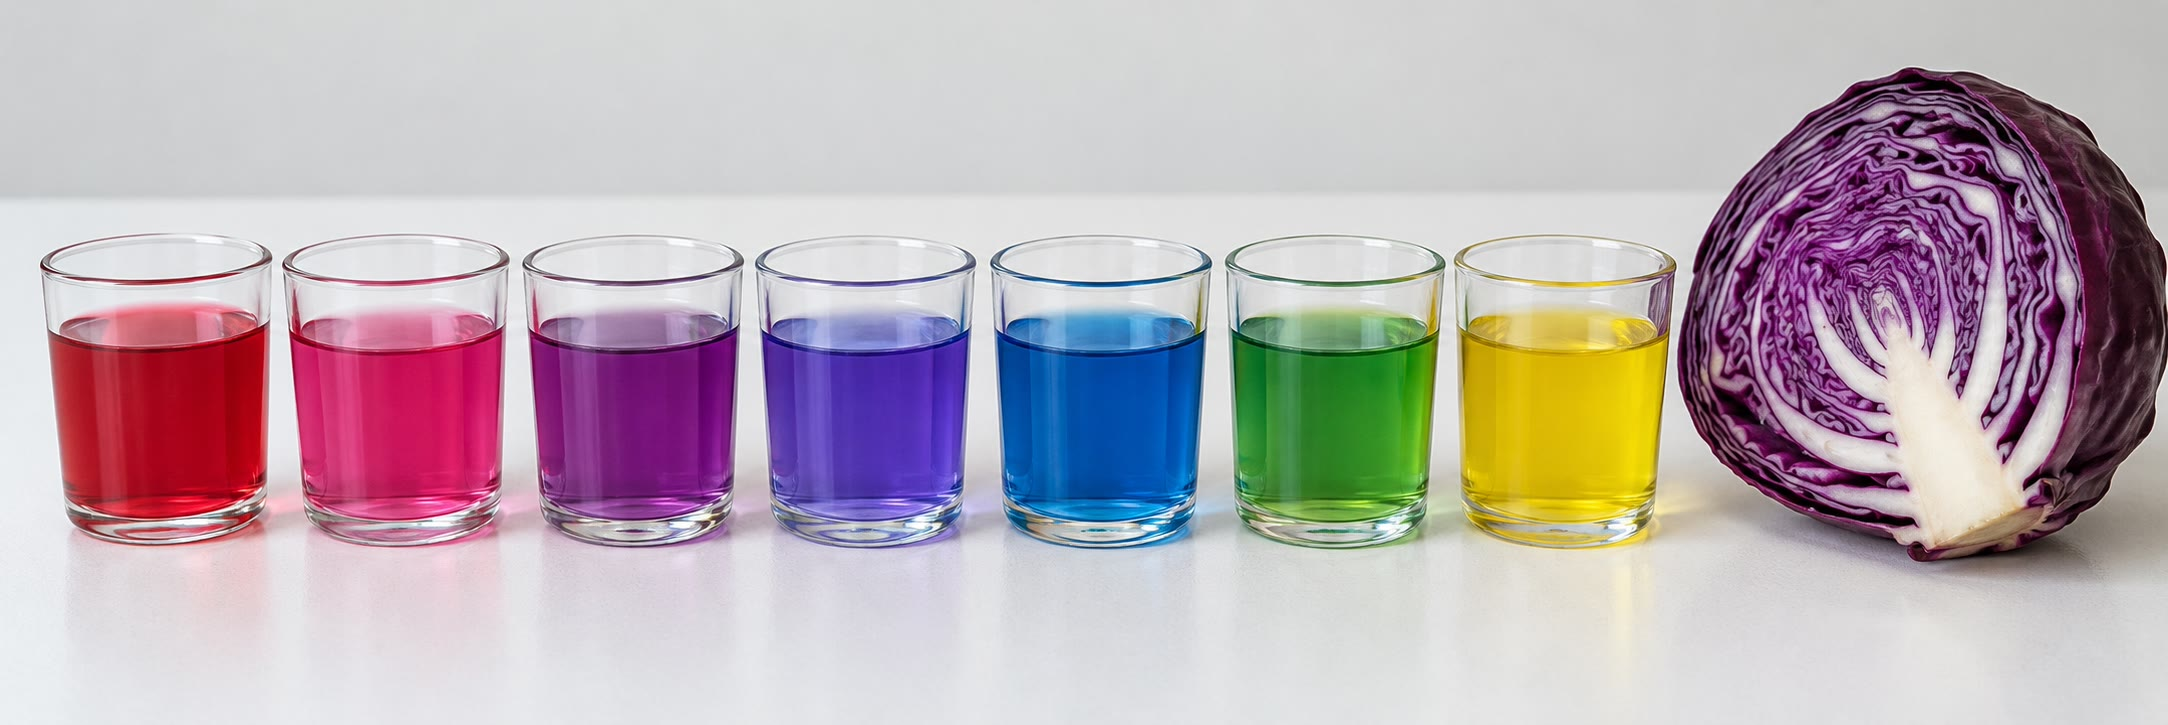
\includegraphics[width=0.55\linewidth]{images/book1/ai/g9-red-cabbage.jpg}

{\small Sari kubis merah, yang disiapkan oleh guru, berubah warna
menurut \omterm{def:g9:acids-bases-ph:ph}{pH}: merah dalam asam, ungu di sekitar netral, biru, hijau, lalu
kuning dalam larutan yang makin lama makin basa.}
\end{omfigure}

\section{Keselamatan dengan produk korosif}

\begin{safety}{\ghs[0.85cm]{GHS05}\ghs[0.85cm]{GHS07}}
% ledger: ghs:HCl, ghs:NaOH
Asam klorida pekat dan natrium hidroksida (basa dalam pembersih saluran)
memuat piktogram korosi GHS05: keduanya menyebabkan luka bakar parah
pada kulit dan mata serta merusak logam. GHS07: iritan. Pakai kacamata
pelindung dan sarung tangan; percikan segera dibilas dengan banyak air.
\end{safety}

\begin{remark}[Jangan pernah mencampur produk pembersih]\label{rem:g9:acids-bases-ph:mix}
Produk yang bersifat asam dan basa bereaksi satu sama lain, kadang-kadang
dengan hebat, dan beberapa \omterm{def:g6:pure-substances-and-mixtures:mixture}{campuran} melepaskan gas beracun: pemutih yang
\omterm{def:g2:mixing-and-dissolving:mix}{dicampur} pembersih kerak yang asam melepaskan klorin. Produk pembersih
tidak pernah \omterm{def:g2:mixing-and-dissolving:mix}{dicampur}.
\end{remark}

\section{Latihan}

\begin{exercise}[$\star$]\label{exo:g9:acids-bases-ph:1}
Asam, basa, atau netral? Larutan \omterm{def:g9:acids-bases-ph:ph}{ber-pH} 3, larutan \omterm{def:g9:acids-bases-ph:ph}{ber-pH} 7, larutan
\omterm{def:g9:acids-bases-ph:ph}{ber-pH} 11.
\end{exercise}

\begin{exercise}[$\star$]\label{exo:g9:acids-bases-ph:2}
\omterm{def:g9:ions:ion}{Ion} mana yang lebih banyak dalam \omterm{def:g9:acids-bases-ph:acidic}{larutan asam}? Dalam \omterm{def:g9:acids-bases-ph:acidic}{larutan basa}?
\end{exercise}

\begin{exercise}[$\star$]\label{exo:g9:acids-bases-ph:3}
Dengan skala \omterm{def:g9:acids-bases-ph:ph}{pH} dalam bab ini, urutkan dari yang paling asam sampai yang
paling basa: kopi, air laut, air jeruk nipis, amonia rumah tangga, air
murni.
\end{exercise}

\begin{exercise}[$\star$]\label{exo:g9:acids-bases-ph:4}
Uraikan cara mengukur \omterm{def:g9:acids-bases-ph:ph}{pH} sebuah larutan dengan \omterm{def:g9:acids-bases-ph:ph-paper}{kertas pH}.
\end{exercise}

\begin{exercise}[$\star\star$]\label{exo:g9:acids-bases-ph:5}
Sebuah larutan \omterm{def:g9:acids-bases-ph:ph}{ber-pH} 4 diencerkan sepuluh kali dengan air. Kira-kira
berapa \omterm{def:g9:acids-bases-ph:ph}{pH-nya} yang baru? Dan jika diencerkan seratus kali?
\end{exercise}

\begin{exercise}[$\star\star$]\label{exo:g9:acids-bases-ph:6}
Dapatkah \omterm{def:g9:acids-bases-ph:acidic}{larutan asam} menjadi basa dengan menambahkan air? Jelaskan.
\end{exercise}

\begin{exercise}[$\star\star$]\label{exo:g9:acids-bases-ph:7}
Mengapa asam harus dituang ke dalam air, dan bukan sebaliknya?
\end{exercise}

\begin{exercise}[$\star\star$]\label{exo:g9:acids-bases-ph:8}
Sebuah botol memuat piktogram GHS05. Apa artinya? Berikan dua tindakan
pencegahan.
\end{exercise}

\begin{exercise}[$\star\star$]\label{exo:g9:acids-bases-ph:9}
Berapa kali pengenceran sepuluh kali lipat yang diperlukan untuk membawa
sebuah asam dari \omterm{def:g9:acids-bases-ph:ph}{pH} 1 ke \omterm{def:g9:acids-bases-ph:ph}{pH} 4? Berapa total pengencerannya?
\end{exercise}

\begin{exercise}[$\star\star$]\label{exo:g9:acids-bases-ph:10}
Susu magnesia diminum untuk mengatasi asam lambung. Dengan skala \omterm{def:g9:acids-bases-ph:ph}{pH},
jelaskan mengapa.
\end{exercise}

\begin{exercise}[$\star\star\star$]\label{exo:g9:acids-bases-ph:11}
\omterm{def:g9:acids-bases-ph:ph}{pH} samudra telah turun sekitar 0.1 sejak era industri. Apakah samudra
sekarang bersifat asam? Ke arah mana \omterm{def:g9:acids-bases-ph:ph}{pH-nya} bergerak, dan mengapa?
\end{exercise}

\begin{exercise}[$\star\star\star$]\label{exo:g9:acids-bases-ph:12}
Seorang siswa mengukur \omterm{def:g9:acids-bases-ph:ph}{pH} cuka yang sama dengan \omterm{def:g9:acids-bases-ph:ph-paper}{kertas pH} (3) dan dengan
\omterm{def:g9:acids-bases-ph:ph-paper}{pH meter} (2.6). Jelaskan mengapa kedua hasil itu berbeda dan mana yang
lebih teliti.
\end{exercise}

\section{Soal: Asam yang Tumpah}

\begin{problem}[{Soal akhir pekan --- satu liter asam yang tumpah di bak
cuci laboratorium, dan mengapa mengencerkannya bukan jawabannya}]
\label{pb:g9:acids-bases-ph:1}
Sebuah botol berisi \qty{1}{L} asam klorida encer, \omterm{def:g9:acids-bases-ph:ph}{ber-pH} 2, pecah di bak
cuci laboratorium. Saluran pembuangan tidak boleh menerima larutan apa
pun yang \omterm{def:g9:acids-bases-ph:ph}{pH-nya} di bawah 5. Pakailah aturan dalam bab ini: untuk asam
ini, setiap pengenceran sepuluh kali lipat menaikkan \omterm{def:g9:acids-bases-ph:ph}{pH} satu satuan.

\medskip
\noindent\textbf{Bagian I --- Asamnya.}
\begin{enumerate}
  \item Apakah larutan itu asam, netral, atau basa? \omterm{def:g9:ions:ion}{Ion} apa yang paling
        banyak dikandungnya?
  \item Piktogram apa yang seharusnya ada pada botol itu, dan mengapa?
  \item Guru mengukur \omterm{def:g9:acids-bases-ph:ph}{pH} dengan \omterm{def:g9:acids-bases-ph:ph-paper}{pH meter} alih-alih dengan \omterm{def:g9:acids-bases-ph:ph-paper}{kertas pH}.
        Berikan satu keuntungannya.
  \item Berapa kali lebih banyak \omterm{def:g9:ions:ion}{ion} \ce{H+} dalam satu liter \omterm{def:g9:acids-bases-ph:ph}{ber-pH} 2
        dibandingkan dalam satu liter \omterm{def:g9:acids-bases-ph:ph}{ber-pH} 3 dari asam yang sama?
\end{enumerate}

\medskip
\noindent\textbf{Bagian II --- Mengencerkan.}
\begin{enumerate}[resume]
  \item Berapa volume larutan yang diperoleh dengan mengencerkan satu
        liter asam itu sepuluh kali? Berapa \omterm{def:g9:acids-bases-ph:ph}{pH-nya}?
  \item Berapa kali pengenceran sepuluh kali lipat yang diperlukan untuk
        mencapai \omterm{def:g9:acids-bases-ph:ph}{pH} 5?
  \item Berapa volume total larutan yang akan dihasilkan?
  \item Dapatkah air sebanyak apa pun membuat larutan itu menjadi basa?
        Jelaskan.
\end{enumerate}

\medskip
\noindent\textbf{Bagian III --- Cara yang lebih baik.}
Sebagai gantinya, guru menambahkan sedikit demi sedikit larutan sebuah
basa sampai \omterm{def:g9:acids-bases-ph:ph-paper}{kertas pH} menunjukkan 7: \omterm{def:g9:ions:ion}{ion-ion} \ce{H+} dari asam bereaksi
dengan \omterm{def:g9:ions:ion}{ion-ion} \ce{OH-} dari basa.
\begin{enumerate}[resume]
  \item Tuliskan \omterm{def:g8:balanced-equations:equation}{persamaan reaksi} antara \omterm{def:g9:ions:ion}{ion} \ce{H+} dan \omterm{def:g9:ions:ion}{ion} \ce{OH-}.
  \item Mengapa cara ini lebih baik daripada mengencerkan?
  \item Sebutkan sebuah produk rumah tangga yang bersifat basa yang dapat
        dipakai di dapur untuk membersihkan tumpahan kecil cuka.
  \item Hitung volume air yang harus ditambahkan ke satu liter asam itu
        untuk membawanya ke \omterm{def:g9:acids-bases-ph:ph}{pH} 5.
\end{enumerate}
\end{problem}
